\documentclass[11pt,a4paper]{article}
\usepackage[utf8]{inputenc}
\usepackage{a4wide}
\usepackage{amsmath}
\usepackage{amsfonts}
\usepackage{amssymb}
\usepackage{graphicx}

\title{Distance and curvature}
\author{Hugues Talbot}

\begin{document}
\maketitle
	
	
	\section{Normals and curvature}
	
	There is a deep link between the evolution of the normal along a curve and the curvature.
	
	Let $C$ be a planar curve. To define the curvature at a point, we can consider
	the case of a straight line. We can admit that in this case the curvature is zero along the line. For a portion of a circle, the curvature is defined to be inversely proportional to the radius of the circle:
	
	\begin{equation}
	\kappa = \frac{1}{R}
	\end{equation}
	
		\begin{figure}
			\centering
			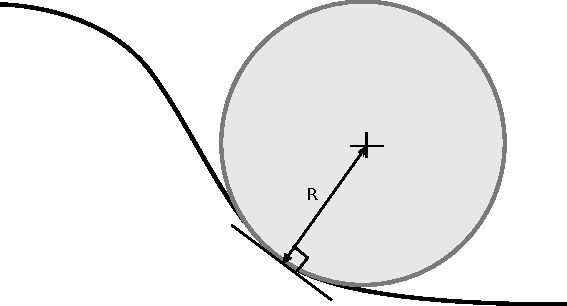
\includegraphics[width=0.5\textwidth]{Drawings/Osculating.pdf}
			\caption{The notion of an osculating circle (best local approximation) defines the curvature as the inverse of the radius of the circle.\label{fig:oscul}}
		\end{figure}
	
	More precisely, for any curve, we can locally approximate a sufficiently regular curve (${\cal C}^2$ is enough) at a point by a circle that best approximates it locally (see Fig.~\ref{fig:oscul}. This circle is tangent to $C$ and is called an {\em osculating circle}. The radius of this circle defines the curvature.
	

	
	Another way to define the curvature is to consider a point moving at a constant speed along the curve $C$. The variation of the tangent vector along the curve defines the curvature. This is equivalent to specifying the acceleration of the point.
	
	\begin{equation}
	\kappa = \frac{d \mathbf{T}}{ds},
	\end{equation}
	
	where $s$ is a parametrisation of the curve. Both definition of the curvature
	are in fact equivalent (see Fig.~\ref{fig:theta}). 
	
	\begin{figure}
		\centering
		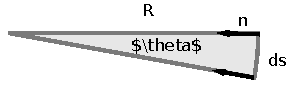
\includegraphics[width=0.3\textwidth]{Drawings/theta.pdf}
		\caption{We can write $\sin d\theta \approx d\theta = \frac{ds}{R}$. As ds tends to zero, we have $R = \frac{d\theta}{ds} = \frac{d \mathbf{T}}{ds}$.\label{fig:theta}}
	\end{figure}
	
	\begin{figure}
		\centering
		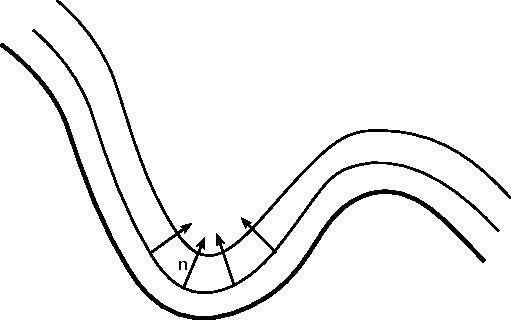
\includegraphics[width=0.5\textwidth]{Drawings/Distance.pdf}
		\caption{The faster the normal evolves along a curve, the higher the curvature.}
	\end{figure}
	
\end{document}